%\documentclass[honours,12pt,twoside]{unswthesis}

\usepackage{afterpage}
\usepackage{amsfonts}
\usepackage{amsmath}
\usepackage{amssymb}
\usepackage{amsthm}
\usepackage[english]{babel}
\usepackage{graphicx}
\usepackage{natbib}
\usepackage[utf8]{inputenc}
\usepackage{latexsym}
\usepackage{url}
\usepackage{todonotes}
\usepackage{tikz}
\usepackage{pdfpages}
\usetikzlibrary{arrows}
\usepackage{float}

\usepackage{booktabs}
\renewcommand{\arraystretch}{1.2}


%%%%%%%%%%%%%%%%%%%%%%%%%%%%%%%%%%%%%%%%%%%%%%%%%%%%%%%%%%%%%%%%%
%
%  The following are some simple LaTeX macros to give some
%  commonly used letters in funny fonts. You may need more or less of
%  these
%
\newcommand{\R}{\mathbb{R}}
\newcommand{\Q}{\mathbb{Q}}
\newcommand{\C}{\mathbb{C}}
\newcommand{\N}{\mathbb{N}}
\newcommand{\F}{\mathbb{F}}
\newcommand{\PP}{\mathbb{P}}
\newcommand{\T}{\mathbb{T}}
\newcommand{\Z}{\mathbb{Z}}
\newcommand{\B}{\mathfrak{B}}
\newcommand{\BB}{\mathcal{B}}
\newcommand{\M}{\mathfrak{M}}
\newcommand{\X}{\mathfrak{X}}
\newcommand{\Y}{\mathfrak{Y}}
\newcommand{\CC}{\mathcal{C}}
\newcommand{\E}{\mathbb{E}}
\newcommand{\cP}{\mathcal{P}}
\newcommand{\cS}{\mathcal{S}}
\newcommand{\A}{\mathcal{A}}
\newcommand{\ZZ}{\mathcal{Z}}

%%%%%%%%%%%%%%%%%%%%%%%%%%%%%%%%%%%%%%%%%%%%%%%%%%%%%%%%%%%%%%%%%%%%%
%
% The following are much more esoteric commands that I have left in
% so that this file still processes. Use or delete as you see fit
%
\newcommand{\bv}[1]{\mbox{BV($#1$)}}
\newcommand{\comb}[2]{\left(\!\!\!\begin{array}{c}#1\\#2\end{array}\!\!\!\right)
}
\newcommand{\Lat}{{\rm Lat}}
\newcommand{\var}{\mathop{\rm var}}
\newcommand{\Pt}{{\mathcal P}}
\def\tr(#1){{\rm trace}(#1)}
\def\Exp(#1){{\mathbb E}(#1)}
\def\Exps(#1){{\mathbb E}\sparen(#1)}
\newcommand{\floor}[1]{\left\lfloor #1 \right\rfloor}
\newcommand{\ceil}[1]{\left\lceil #1 \right\rceil}
\newcommand{\hatt}[1]{\widehat #1}
\newcommand{\modeq}[3]{#1 \equiv #2 \,(\text{mod}\, #3)}
\newcommand{\rmod}{\,\mathrm{mod}\,}
\newcommand{\p}{\hphantom{+}}
\newcommand{\vect}[1]{\mbox{\boldmath $ #1 $}}
\newcommand{\reff}[2]{\ref{#1}.\ref{#2}}
\newcommand{\psum}[2]{\sum_{#1}^{#2}\!\!\!'\,\,}
\newcommand{\bin}[2]{\left( \begin{array}{@{}c@{}}
				#1 \\ #2
			\end{array}\right)	}
%
%  Macros - some of these are in plain TeX (gasp!)
%
\newcommand{\be}{($\beta$)}
\newcommand{\eqp}{\mathrel{{=}_p}}
\newcommand{\ltp}{\mathrel{{\prec}_p}}
\newcommand{\lep}{\mathrel{{\preceq}_p}}
\def\brack#1{\left \{ #1 \right \}}
\def\bul{$\bullet$\ }
\def\cl{{\rm cl}}
\let\del=\partial
\def\enditem{\par\smallskip\noindent}
\def\implies{\Rightarrow}
\def\inpr#1,#2{\t \hbox{\langle #1 , #2 \rangle} \t}
\def\ip<#1,#2>{\langle #1,#2 \rangle}
\def\lp{\ell^p}
\def\maxb#1{\max \brack{#1}}
\def\minb#1{\min \brack{#1}}
\def\mod#1{\left \vert #1 \right \vert}
\def\norm#1{\left \Vert #1 \right \Vert}
\def\paren(#1){\left( #1 \right)}
\def\qed{\hfill \hbox{$\Box$} \smallskip}
\def\sbrack#1{\Bigl \{ #1 \Bigr \} }
\def\ssbrack#1{ \{ #1 \} }
\def\smod#1{\Bigl \vert #1 \Bigr \vert}
\def\smmod#1{\bigl \vert #1 \bigr \vert}
\def\ssmod#1{\vert #1 \vert}
\def\sspmod#1{\vert\, #1 \, \vert}
\def\snorm#1{\Bigl \Vert #1 \Bigr \Vert}
\def\ssnorm#1{\Vert #1 \Vert}
\def\sparen(#1){\Bigl ( #1 \Bigr )}

\newcommand\blankpage{%
    \null
    \thispagestyle{empty}%
    \addtocounter{page}{-1}%
    \newpage}
    
%%%%%%%%%%%%%%%%%%%%%%%%%%%%%%%%%%%%%%%%%%%%%%%%%%%%%%%%%%%%%%
%
% These environments allow you to get nice numbered headings
%  for your Theorems, Definitions etc.  
%
%  Environments
%
%%%%%%%%%%%%%%%%%%%%%%%%%%%%%%%

\newtheorem{theorem}{Theorem}[section]
\newtheorem{lemma}[theorem]{Lemma}
\newtheorem{proposition}[theorem]{Proposition}
\newtheorem{corollary}[theorem]{Corollary}
\newtheorem{conjecture}[theorem]{Conjecture}
\newtheorem{definition}[theorem]{Definition}
\newtheorem{example}{Example}
\newtheorem{remark}[theorem]{Remark}
\newtheorem{question}[theorem]{Question}
\newtheorem{notation}[theorem]{Notation}
\numberwithin{equation}{section}

%\begin{document}

\chapter{Convolutional neural networks}\label{convnets}

Convolutional neural networks (CNNs) are of particular interest when working with image problems. The input data is assumed to be in 2 dimensions. Unlike fully connected layers, convolutional layers look to identify particular features within a subset of the 2D data sample. Collections of these features can be combined and interpreted for image classification.

% Diagram of typical CNN structure
\begin{figure}[ht]
	\centering
	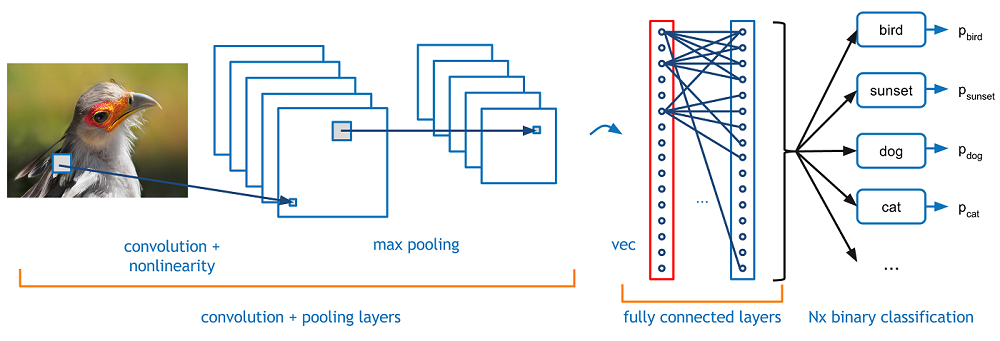
\includegraphics[width=\textwidth]{Images/4_cnn_structure.png}
	\caption{Typical CNN Structure. Convolution layers, with ReLU activation (nonlinearity), are followed by pooling layers. Final layers are fully connected, using softmax activation.}
	\small Image taken from \cite{ADeshpande2016}
	\label{convnets-structurefig}
\end{figure}

As shown in Figure \ref{convnets-structurefig}, CNNs typically consist of alternating convolutional layers (Section \ref{convnets-convlayer}) and max pooling layers (Section \ref{convnets-pool}). For classification tasks, the last layers of the network are fully connected. Softmax activation is used for the final output layer, to generate a probability distribution as with other classification tasks.

\section{Convolutional layers}\label{convnets-convlayer}

In a convolutional layer, a \textit{filter} is a matrix of weights that describes a particular visual feature to be identified. These filters have predetermined dimensions, usually set to assess a small subset of the original image. Each filter has the same depth as the original image. For instance, an image that has three colour channels; red, blue and green, will have convolution filters also with a depth of three. Each convolutional layer can have many filters.

The filters are then said to \textit{convolve} around the image. Suppose that a filter $F^{(f)}$ has dimension $M\times N \times C$. Given an input image matrix $X$, the value of the convolution at element $X_{j,k}$ is given by
\[
	a_{jk}^{(f)} = \sigma\bigg(\sum_{c=1}^C\sum_{m=0}^{M-1}\sum_{n=0}^{N-1}X_{j+m, k+n, c}F_{m,n,c}^{(f)}  + b^{(f)}\bigg)
\]
where $\sigma(\cdot)$ is some activation function as before, $C$ is the number of input channels and $b^{(f)}$ is the bias to be added when using filter $f$. 

% Diagram of convolution algorithm
\begin{figure}[ht]
	\centering
	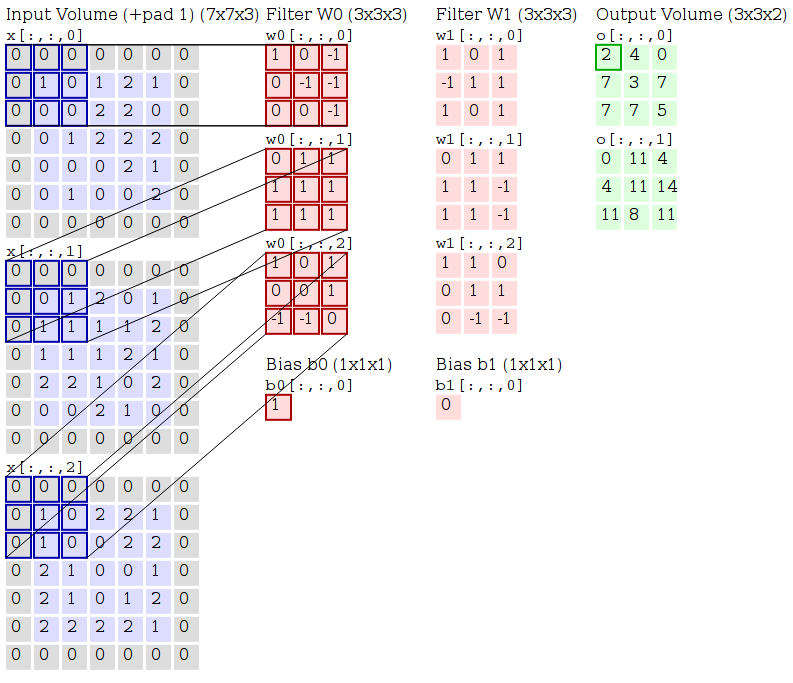
\includegraphics[scale=0.5]{Images/4_convolution.png}
	\caption{Convolution algorithm with 2 filters of size 3x3, stride 2, zero padding 1}
	\small Image adapted from \url{'http://cs231n.github.io/convolutional-networks/'}
	\label{convnets-conv-alg}
\end{figure}

As shown in Figure \ref{convnets-conv-alg}, the convolution process starts from the top-left corner of the input volume. A subset of the image is taken at that location, with the same dimensions as the filter. The image subset and the filter are point-wise multiplied and added together. A bias variable is added and an activation function applied as with fully connected layers. This result becomes the output of a single neuron of the convolutional layer. The filter is moved to the next location (depending on the size of the stride) to build the value of the next neuron.

Each filter of a convolutional layer builds a matrix of neurons, where its dimension is a subset of the original image (depending on the size of the zero padding). These matrices are bound together to form a 3D array, with depth depending on the number of filters used.

\subsection*{Zero padding}\label{convnets-pad}

As the filters convolve around the image, the filters can only be placed within the bounds of the input image. This results in some loss of dimension. For a starting image with dimension $J \times K$ and a filter with dimension $M \times N$, the convolutional output will be of dimension $(J - M + 1)\times (K - N + 1)$.

In order to retain the original image dimensions, the input image can be zero padded, with padding given by $P$. The dimension of the original image is increased to $(J+2P) \times (K+2P)$, with the outer $P$ elements all set to zero. When the convolution takes place, the resulting image size will have dimension $(J+2P - M + 1) \times (K + 2P - N + 1)$.

\subsection*{Stride}\label{convnets-stride}

As the dimension of images an be quite large, moving a convolutional filter by only one element at a time can make the training process very long. To reduce the number of resulting variables, the filter can be moved by multiple elements at a time. The distanced moved is known as the \textit{stride}, given by $S$.

For an input image with dimension $J \times K$, a filter with dimension $M \times N$, with padding $P$ and stride $S$, the output given by convolution will have dimension $\Big(\Bigl\lfloor \dfrac{J + 2P - M}{S}\Bigr\rfloor + 1\Big) \times \Big(\Bigl\lfloor \dfrac{K + 2P - N}{S} \Bigr\rfloor + 1\Big)$.

\section{Pooling layers}\label{convnets-pool}

It is common practise to follow convolution layers with max pooling layers. Pooling is a method of dimension reduction. Pooling layers create a sliding window of specified dimension and stride size. At each sliding window position, the pooling layer outputs a single value. In particular for max pooling, the layer outputs the maximum value at each sliding window location.

The motivation behind this is that convolutional layers output high values in regions where the features of interest have been located. However, the algorithm is only interested in gathering information for classification and does not need the location to be highly specific. To improve computation time, it is then advantageous to remove a large number of variables, while retaining variables that identify significant features.

\section{ReLU activation}\label{convnets-act}

The ReLU activation function, as defined in Section \ref{nnets-act}, is frequently used for  convolutional neural networks. As image data presents a very large number of variables, computation time can become very large. To aid this, the ReLU function is a common choice, as it can be computed very quickly. Additionally, the ReLU activation function is also able to avoid the vanishing gradient problem (see Section \ref{nnet-vanishinggradprob}.


%Convolutional Neural Networks are very similar to traditional neural networks, but make the assumption that the input data are images.
%The neurons of a convNet are arranged in 3D. 
%http://cs231n.github.io/convolutional-networks/
%
%Input layer: raw pixel values, with width, height and color channels
%Conv layer: Compute output for regions of input. Each computes a dot product between weights and a region that they are connected to.
%ReLU: elementwise activation function.
%Pool: downsampling
%FC - fully connected: each neuron here is connected to all previous.
%
%Conv layer has a set of learnable filters. The filter might have only a small size, but will slide (convolve) across the image, computing dot products at each position.

%https://stats.stackexchange.com/questions/154879/a-list-of-cost-functions-used-in-neural-networks-alongside-applications
%https://pappubahry.com/misc/neural/nielsen_1/
% http://neuralnetworksanddeeplearning.com/

%Good animated representation: https://ujjwalkarn.me/2016/08/11/intuitive-explanation-convnets/
%
%https://medium.com/technologymadeeasy/the-best-explanation-of-convolutional-neural-networks-on-the-internet-fbb8b1ad5df8
%
%https://tensorflow.rstudio.com/tensorflow/articles/tutorial_mnist_beginners.html
%
%https://adeshpande3.github.io/A-Beginner%27s-Guide-To-Understanding-Convolutional-Neural-Networks-Part-2/
%
%https://tech.hbc.com/2016-05-18-fully-connected-to-convolutional-conversion.html


%\section{R-CNN}
%Purpose is to take in an image, and draw bounding boxes over all of the objects. Train to find 4D output (x, y, width, height) of object. Use L2 distance loss between prediction and 'ground truth'.
%
%Done by attaching a fully connected layer to the last conv layer. Separate classification layers and box coord layers. 
%Accuracy determined by Intersection over Union (ioU) area. 






%%%%%%%%%%%%%%%%%%%%%%%%%%%%%%%%%%%%%%%%%%%%%%%%%%%%%%%%%%%%%%%%%%%%%%%%%%%

%\clearpage

\addcontentsline{toc}{chapter}{References}

\bibliographystyle{apalike}
\bibliography{bibliography.bib}

%\bibliographystyle{apacite}
%\bibliography{mybib.bib}

